\documentclass[14pt]{beamer}
\usetheme{Luebeck} %Malmoe

\usepackage[english]{babel}
\usepackage[latin1]{inputenc}
\title[Construction of GNU Compiler Collection Front End]{Construction of GNU Compiler Collection Front End}

\author[Petr Machata]{Petr Machata \\ \texttt{xmacha31@stud.fit.vutbr.cz}}
\date{2007-01-09}

\def\Algol{{\sc Algol}\space}

\begin{document}

\frame{\titlepage}

\frame
{
  \frametitle{About My Project}

  \begin{itemize}
  \item The goal: GCC Front End Howto
  \item The side effect: write \Algol 60 compiler
  \item Personal ambition: general usefulness
    \begin{itemize}
    \item English, Open Source
    \end{itemize}
  \item Exploit GCC
    \begin{itemize}
    \item Inline assembly, attributes, OpenMP
    \item CPP, runtime library
    \end{itemize}
  \end{itemize}
}

\iffalse
\frame
{
  \frametitle{GCC Architecture}

  \begin{itemize}
  \item Driver vs. Proper; lang-specific driver
  \item Front end, Middle end, Back end; hooks
  \item GENERIC, GIMPLE; C expressiveness; AST
  \item Garbage collector
  \end{itemize}
}
\fi
\frame
{
  \frametitle{GCC Architecture}

  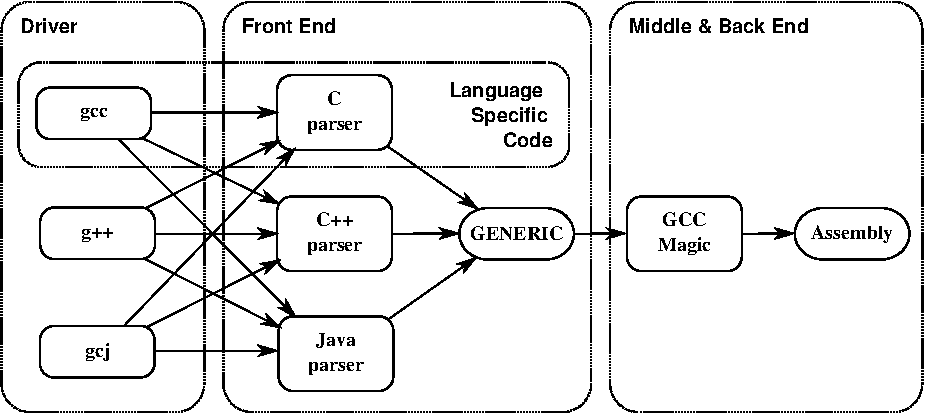
\includegraphics[height=4.8cm]{demo-gccarch.pdf}
}

\frame
{
  \frametitle{Summay of a Work}

  \begin{itemize}
  \item {\tt al60l} can parse most of \Algol 60
    \begin{itemize}
    \item No functions \& extensions yet
    \end{itemize}
  \item {\tt ga60} compiles simple programs
    \begin{itemize}
    \item Loops, compounds, variables, simple goto
    \item Runtime library: \texttt{puts}, \texttt{exit}, \texttt{**}.
    \end{itemize}
  \item Plenty of work still ahead
    \begin{itemize}
    \item Functions, static variables, ...
    \item Bootstrapping; both library and frontend
    \item Crosscompilation
    \end{itemize}
  \end{itemize}
}

\end{document}

% Local Variables:
% compile-command: "make show-demo-1"
% End:
